\documentclass[UTF8,a4paper,fontset=fandol,zihao=5]{ctexart}
\usepackage[margin=2cm,top=1.8cm,bottom=1.8cm]{geometry}
\usepackage{amsmath,amssymb,graphicx,array,xcolor,colortbl,url,hyperref}
\hypersetup{hidelinks,pdftitle={小车倒立摆的离散PID与LQR控制性能比较}}
\setmainfont{texgyretermes-regular.otf}[BoldFont=texgyretermes-bold.otf,ItalicFont=texgyretermes-italic.otf,BoldItalicFont=texgyretermes-bolditalic.otf]
\definecolor{tablehead}{RGB}{233,238,243}
\definecolor{tableborder}{RGB}{217,217,217}
\pagestyle{plain}
\setlength{\parindent}{2em}
\setlength{\parskip}{2pt}
\setlength{\abovedisplayskip}{4pt}
\setlength{\belowdisplayskip}{4pt}
\setlength{\abovedisplayshortskip}{3pt}
\setlength{\belowdisplayshortskip}{3pt}
\ctexset{section={format=\large\bfseries,beforeskip=5pt,afterskip=4pt},
subsection={format=\normalsize\bfseries,beforeskip=5pt,afterskip=4pt}}
\begin{document}
\linespread{1}
\fontsize{10.5}{14}\selectfont

\begin{center}{\fontsize{17}{23}\selectfont\bfseries 小车倒立摆的离散PID与LQR控制性能比较}\end{center}
\subsection*{摘要}
小车倒立摆具有非线性、欠驱动和直立平衡点不稳定等特点，是研究计算机控制的典型对象。本文建立连续非线性模型，在直立点附近设计串级PID与离散LQR，并在同一非线性对象、采样周期和执行器力限制下比较性能。PID通过完整五阶闭环系数匹配确定增益，LQR通过零阶保持离散化及离散Riccati方程得到反馈增益。12次无噪声初态仿真表明，两种方法均能恢复5°—30°的初始偏角，LQR调节时间缩短约26.0\%—43.0\%，最大位置偏移和控制力平方积分均更小。1440次带噪仿真中，LQR在输入端噪声下的末段摆角RMS约降低56.7\%，在传感器噪声下约降低26.5\%，但后者的执行器力RMS约增加64.0\%。本文的亮点是将统一非线性验证、同种子噪声配对和控制用力评价结合起来，保留性能收益与代价，形成可复现的比较流程。\par
\par\noindent{\fontsize{8.7}{11}\selectfont 关键词  小车倒立摆；离散控制；串级PID；LQR；噪声鲁棒性}\par
\section*{1 前言}
\subsection*{1.1 背景与研究意义}
倒立摆只有作用于小车的一个水平输入，却需要同时调节小车位置和摆杆姿态。直立点附近的微小偏差会不断放大，而较大的控制动作又可能带来较大行程或触发执行器饱和，因此适合用于分析稳定性、动态响应与输入约束之间的关系。\par
在计算机控制中，状态读取和控制更新是离散进行的，被控对象却持续运动。连续线性模型中的稳定极点只能描述局部设计性质；实际表现还受到采样周期、积分时序、输入保持、非线性和测量误差的影响。本文将这些实现细节纳入同一仿真框架。\par
\subsection*{1.2 研究目标与比较原则}
本文比较基于传递函数的串级PID与基于状态空间的离散LQR。两者均可获得位置、速度、摆角和角速度四个状态，差异来自控制结构和固定参数，而非传感器信息数量不同。比较先考察不同初始摆角下的恢复过程，再考察输入端随机外力和传感器噪声下的状态波动及控制用力。\par
全文以当前固定PID极点和LQR权重为主线。模型、初态、反馈周期、执行器力限幅及求解精度保持一致，不按工况重新整定。结论限定于实际测试的初态、噪声范围和有限仿真时域，不将单个优势案例解释为全局稳定性或普遍优越性。\par
\newpage
\section*{2 数学模型}
\subsection*{2.1 对象与坐标约定}
系统由质量为M的小车、无质量刚杆和质量为m的杆端质点组成，支点到质点的距离为L。小车位置p和水平力F向右为正，摆角$\theta$以竖直向上为零，向右倾斜为正。忽略摩擦、空气阻力、电机动态、轨道边界与碰撞。内部采用SI单位及弧度，角度连续累计。\par
\[
x=\begin{bmatrix}p&v&\theta&\omega\end{bmatrix}^{T},\qquad v=\dot p,\quad\omega=\dot\theta.
\]
\par\noindent\begin{minipage}{\linewidth}\centering
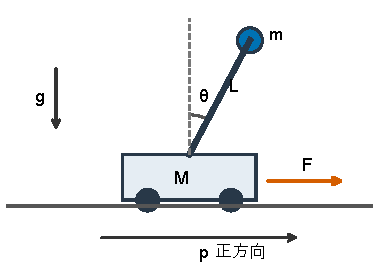
\includegraphics[width=8.0cm]{figures/model.pdf}
\par\vspace{2pt}{\raggedright\fontsize{8.7}{11}\selectfont 图1 小车倒立摆的几何关系及正方向示意。图中姿态用于说明坐标，不代表某次仿真的状态。\par}\end{minipage}\par\vspace{3pt}
\subsection*{2.2 连续非线性动力学}
杆端坐标为(p+L sin$\theta$, L cos$\theta$)。系统动能和势能分别为\par
\[
T=\frac{1}{2}(M+m)v^2+mLv\omega\cos\theta+\frac{1}{2}mL^2\omega^2,\quad V=mgL\cos\theta.
\]
取广义坐标[p, $\theta$]，以F作为小车方向的广义力，由拉格朗日方程得到\par
\[
\begin{aligned}(M+m)\ddot p+mL\cos\theta\ddot\theta-mL\omega^2\sin\theta&=F,\\mL\cos\theta\ddot p+mL^2\ddot\theta-mgL\sin\theta&=0.\end{aligned}
\]
令$\Delta$=M+m sin$^2$$\theta$，解得用于实际仿真的非线性状态方程\par
\[
\begin{aligned}\dot p&=v,\qquad\dot\theta=\omega,\\\dot v&=\frac{F+mL\omega^2\sin\theta-mg\sin\theta\cos\theta}{\Delta},\\\dot\omega&=\frac{(M+m)g\sin\theta-F\cos\theta-mL\omega^2\sin\theta\cos\theta}{L\Delta}.\end{aligned}
\]
机械能E=T+V满足dE/dt=Fv。程序同步积分外力做功，以E(t)$-$E(0)$-$$\int$Fv dt检验数值一致性。直立附近，正力使小车向右加速、摆杆产生负角加速度，后续反馈符号均按此约定。\par
\newpage
\subsection*{2.3 直立点线性化与传递函数}
在直立静止点附近作小扰动线性化，保留一阶项，可得设计用状态空间模型。若输出选为小车位置与摆角，则有\par
\[
\dot x=Ax+BF,\qquad y=Cx,\qquad D=0,
\]
\[
A=\begin{bmatrix}0&1&0&0\\0&0&-mg/M&0\\0&0&0&1\\0&0&(M+m)g/(ML)&0\end{bmatrix},\quad B=\begin{bmatrix}0\\1/M\\0\\-1/(ML)\end{bmatrix},
\]
\[
C=\begin{bmatrix}1&0&0&0\\0&0&1&0\end{bmatrix}.
\]
零初态下，由线性化方程得到输入力到摆角、位置的传递函数\par
\[
G_{\theta}(s)=-\frac{1}{MLs^2-(M+m)g},\quad G_p(s)=\frac{Ls^2-g}{s^2[MLs^2-(M+m)g]}.
\]
角度通道没有包含小车绝对位置和匀速平移模态，不能仅通过角度稳定判断全状态恢复。因此，PID整定采用完整串级闭环，LQR使用完整四维状态。\par
\subsection*{2.4 采样与零阶保持}
控制器在$t_k$=k$T_s$更新，两个采样时刻之间保持输入不变。线性模型采用精确零阶保持离散化[1]：\par
\[
x_{k+1}=A_dx_k+B_du_k,\quad A_d=e^{AT_s},\quad B_d=\int_0^{T_s}e^{A\tau}B\,d\tau.
\]
该离散模型仅用于设计和局部稳定性检查。所有性能检验仍由原始连续非线性方程推进，不以离散线性对象替代非线性对象。\par
\section*{3 控制方法}
\subsection*{3.1 串级PID的离散实现}
外环根据位置误差生成目标倾角，内环根据倾角误差生成水平力。设目标位置r=0，$\operatorname{sat}_a$表示限幅至[$-$a,a]，则\par
\[
\begin{aligned}e_{p,k}&=r-p_k,\\\theta_{r,k}&=\operatorname{sat}_{\theta_{\max}}(K_pe_{p,k}+I_{p,k}-K_dv_k),\\e_{\theta,k}&=\theta_k-\theta_{r,k},\\u_k&=\operatorname{sat}_{u_{\max}}(k_ae_{\theta,k}+I_{\theta,k}+d_a\omega_k).\end{aligned}
\]
\[
I_{k+1}=\operatorname{sat}_{I_{\max}}(I_k+k_iT_se_k),\qquad I_0=0.
\]
两环先用当前积分贡献计算输出，再更新积分供下一拍使用。外环D项直接使用$-$v，内环D项直接使用$\omega$，不使用差分估计，且不包含目标倾角变化率。当前内环ki=0，实际结构为位置PID与摆角PD；仅限制积分项幅值，不实施完整抗饱和回算。\par
\newpage
\subsection*{3.2 PID参数整定与局部稳定性}
四个物理状态与位置积分状态构成五阶闭环。未饱和连续近似的特征多项式为\par
\[
\begin{aligned}D(s)=&s^3[MLs^2+d_as+k_a-(M+m)g]\\&+k_a(g-Ls^2)(K_ds^2+K_ps+K_i).\end{aligned}
\]
选取完整闭环目标极点[$-$1,$-$1.2,$-$1.5,$-$2,$-$2.5]，以ML为首项系数构造目标多项式，按同次幂系数匹配求得两环增益。五个极点属于完整系统，不分别对应两环的独立极点。当前固定参数如下。\par
\par\noindent{\fontsize{8.7}{11}\selectfont 表1 固定PID参数}\par\vspace{3pt}
{\fontsize{9.3}{11.4}\selectfont\setlength{\tabcolsep}{3pt}\renewcommand{\arraystretch}{1.1}\arrayrulecolor{tableborder}\noindent\begin{tabular}{|>{\raggedright\arraybackslash}p{4.437cm}|>{\centering\arraybackslash}p{3.871cm}|>{\centering\arraybackslash}p{3.871cm}|>{\centering\arraybackslash}p{3.871cm}|}\hline
\rowcolor{tablehead}\textbf{环路} & \textbf{kp} & \textbf{ki} & \textbf{kd}\\\hline
位置外环 & 0.046591 & 0.013703 & 0.062439\\\hline
摆角内环 & 33.474817 & 0 & 5.145074\\\hline
\end{tabular}}\par\vspace{3pt}
目标倾角限幅为$\pm$10°，执行器力限幅为$\pm$20 N，位置积分贡献上限为0.05 rad。再依据真实零阶保持及“输出后更新积分”的时序检查增广离散闭环，其谱半径约为0.98379，小于1。这是未饱和局部模型的稳定性检查，不是非线性全局恢复保证。\par
\subsection*{3.3 离散LQR的设计}
LQR在离散模型上最小化无限时域加权二次代价，协调四个状态偏差与控制需求：\par
\[
J=\sum_{k=0}^{\infty}(x_k^TQx_k+u_k^TRu_k),\quad Q=\operatorname{diag}(10,1,100,1),\quad R=1.
\]
由离散代数Riccati方程求得S[2]，继而得到反馈增益K：\par
\[
\begin{aligned}S=&A_d^TSA_d+Q\\&-A_d^TSB_d(R+B_d^TSB_d)^{-1}B_d^TSA_d,\\K=&(R+B_d^TSB_d)^{-1}B_d^TSA_d.\end{aligned}
\]
\[
u_k=\operatorname{sat}_{20}(-Kx_k),\quad K=\begin{bmatrix}-2.72537&-4.26843&-51.07392&-9.04203\end{bmatrix}.
\]
Ts=0.02 s时，离散线性闭环矩阵的极点最大模约为0.98250。K的负号与本文坐标方向一致，正初始倾角会产生正向纠偏力。标准LQR的最优性对应线性、无约束二次代价；加入限幅后，不能将其直接解释为受限非线性系统的全局最优控制。\par
\subsection*{3.4 控制结构与适用边界}
串级PID通过外环组织位置调节，含位置积分；LQR同时反馈四个状态，但未增广位置积分。两者均使用同一组状态信息，噪声实验不另加滤波或状态估计器。固定参数比较反映本组设计的表现，不等价于在所有整定方案中比较算法优劣。\par
对仅有正初始倾角且角速度为零的状态，若0$<$$\theta$$<$90°，使首拍角加速度指向直立需要F$>$(M+m)g tan$\theta$。60°对应约33.98 N，超过20 N限幅，说明局部纠偏能力受约束；这一首拍条件不能单独确定全局吸引域。本文当前参数的正式初态结论仅覆盖5°—30°。\par
\newpage
\section*{4 仿真实验}
\subsection*{4.1 实现方法与评价指标}
仿真采用Python 3.9.12、NumPy 1.24.1和SciPy 1.9.3。统一M=m=1 kg、L=0.5 m、g=9.81 m/s$^2$，反馈周期0.02 s，仿真30 s。各组仅初始摆角非零。DOP853的最大步长与输出间隔均为0.01 s，rtol=10$^{-9}$、atol=10$^{-11}$。每次创建新控制器并从零积分开始，记录真实状态、执行器力、外力和总力。\par
无噪声恢复要求末5 s全部记录满足|p|、|v|$<$0.01（SI单位），|$\theta$|$<$0.1°、|$\omega$|$<$0.1°/s。调节时间$t_s$取首次进入并保持到终点的时刻；另比较最大位置偏移$p_{\max}$和控制力平方积分$E_u$=$\int$u$^2$dt。该平方积分反映控制需求，不直接等于电机能耗。\par
\subsection*{4.2 不同初始摆角下的表现}
\par\noindent\begin{minipage}{\linewidth}\centering
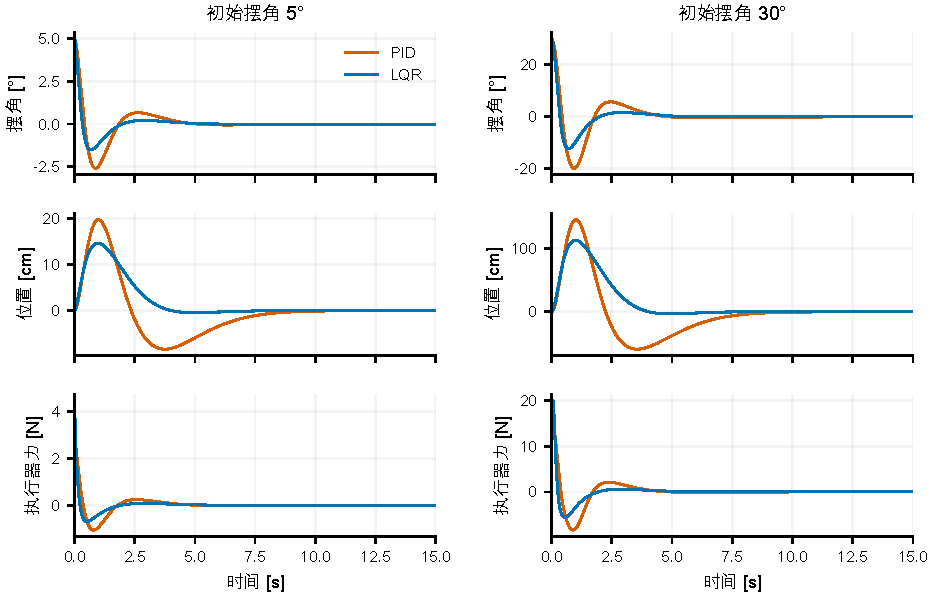
\includegraphics[width=15.4cm]{figures/baseline.pdf}
\par\vspace{2pt}{\raggedright\fontsize{8.7}{11}\selectfont 图2 无噪声下5°与30°初态的响应。图中截取0—15 s以便观察瞬态，评价指标使用完整30 s记录。\par}\end{minipage}\par\vspace{3pt}
\par\noindent{\fontsize{8.7}{11}\selectfont 表2 六组初态的调节时间与最大位置偏移}\par\vspace{3pt}
{\fontsize{9.3}{11.4}\selectfont\setlength{\tabcolsep}{3pt}\renewcommand{\arraystretch}{1.1}\arrayrulecolor{tableborder}\noindent\begin{tabular}{|>{\raggedright\arraybackslash}p{2.360cm}|>{\centering\arraybackslash}p{4.532cm}|>{\centering\arraybackslash}p{4.532cm}|>{\centering\arraybackslash}p{4.626cm}|}\hline
\rowcolor{tablehead}\textbf{初始摆角} & \textbf{LQR表现} & \textbf{PID表现} & \textbf{两者差距}\\\hline
5° & 4.32 s\newline 0.146 m & 7.58 s\newline 0.197 m & 快 3.26 s\newline 位移低 0.051 m\\\hline
10° & 5.21 s\newline 0.296 m & 8.37 s\newline 0.400 m & 快 3.16 s\newline 位移低 0.104 m\\\hline
15° & 5.74 s\newline 0.456 m & 8.80 s\newline 0.618 m & 快 3.06 s\newline 位移低 0.162 m\\\hline
20° & 6.13 s\newline 0.631 m & 9.10 s\newline 0.858 m & 快 2.97 s\newline 位移低 0.227 m\\\hline
25° & 6.60 s\newline 0.837 m & 9.31 s\newline 1.130 m & 快 2.71 s\newline 位移低 0.293 m\\\hline
30° & 6.99 s\newline 1.127 m & 9.45 s\newline 1.451 m & 快 2.46 s\newline 位移低 0.324 m\\\hline
\end{tabular}}\par\vspace{3pt}
\par\noindent{\fontsize{8.7}{11}\selectfont 注：表现列第一行为$t_s$，第二行为$p_{\max}$；差距均以PID为参照，基于未舍入数据计算。}\par
六组初态下，两种方法均达标。LQR调节时间缩短约26.0\%—43.0\%，最大位置偏移均更小。以30°为例，LQR最大位移为1.127 m，PID为1.451 m；控制力平方积分分别为75.22与98.32 N$^2$·s，LQR约低23.49\%。图2还显示其反向摆动较小。\par
\newpage
\subsection*{4.3 输入端噪声下的鲁棒性}
从t=0开始，在执行器限幅后叠加随机水平外力$d_k$，总力$F_k$=$u_k$+$d_k$。$d_k$在每个采样时刻独立生成并保持一拍，服从U($-$0.5$\alpha$,0.5$\alpha$) N；$\alpha$=0.5、1、2分别对应$\pm$0.25、$\pm$0.5、$\pm$1 N。本项实验无测量噪声。\par
两类噪声均覆盖六初态、三强度和20个随机种子，同种子下PID与LQR共用相同序列。全部实验为12次无噪声基准及1440次带噪仿真，共1452次。不同初态复用噪声，统计时不将六初态池化为更多独立样本。\par
\par\noindent\begin{minipage}{\linewidth}\centering
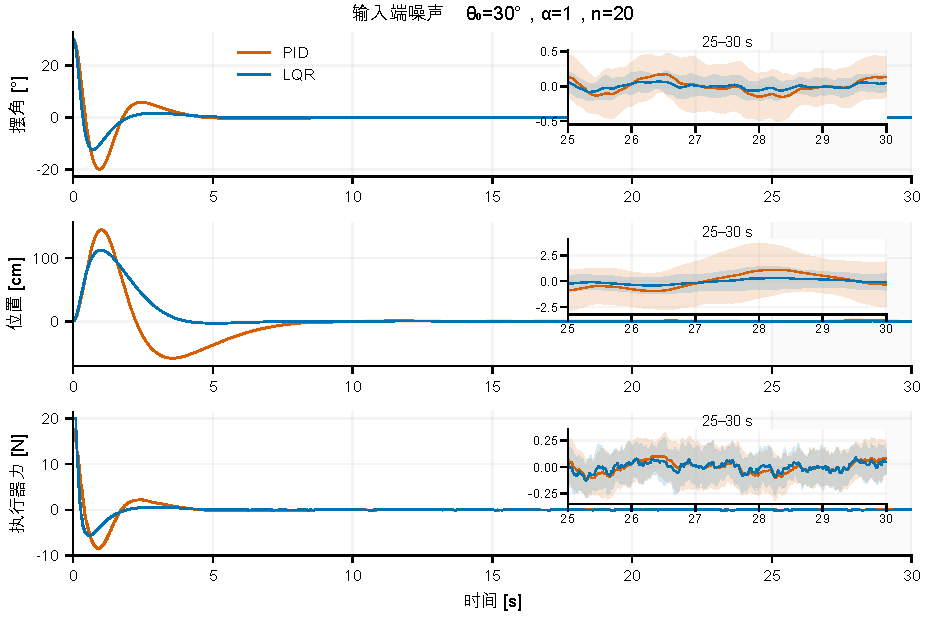
\includegraphics[width=15.8cm]{figures/noise_input.pdf}
\par\vspace{2pt}{\raggedright\fontsize{8.7}{11}\selectfont 图3 输入端噪声下的响应（$\theta_0$=30°，$\alpha$=1，n=20）。实线为均值，阴影为$\pm$1样本标准差，非置信区间；插图放大25—30 s。\par}\end{minipage}\par\vspace{3pt}
\par\noindent{\fontsize{8.7}{11}\selectfont 表3 标准输入端噪声下的末段RMS比较}\par\vspace{3pt}
{\fontsize{9.3}{11.4}\selectfont\setlength{\tabcolsep}{3pt}\renewcommand{\arraystretch}{1.1}\arrayrulecolor{tableborder}\noindent\begin{tabular}{|>{\raggedright\arraybackslash}p{4.249cm}|>{\centering\arraybackslash}p{3.965cm}|>{\centering\arraybackslash}p{3.965cm}|>{\centering\arraybackslash}p{3.871cm}|}\hline
\rowcolor{tablehead}\textbf{评价指标} & \textbf{LQR表现} & \textbf{PID表现} & \textbf{两者差距}\\\hline
摆角 RMS（°） & 0.1355 $\pm$ 0.0255 & 0.3126 $\pm$ 0.0679 & 降低 56.67\%\\\hline
位置 RMS（cm） & 0.8136 $\pm$ 0.2607 & 2.0178 $\pm$ 0.6005 & 降低 59.68\%\\\hline
执行器力 RMS（N） & 0.1634 $\pm$ 0.0173 & 0.1871 $\pm$ 0.0348 & 降低 12.69\%\\\hline
\end{tabular}}\par\vspace{3pt}
\par\noindent{\fontsize{8.7}{11}\selectfont 注：数值为20种子的均值$\pm$样本标准差，统计窗口为25—30 s，位置与摆角均取真实状态。}\par
标准输入噪声下，LQR摆角RMS从PID的0.3126°降至0.1355°，降低56.67\%；位置RMS降低59.68\%，执行器力RMS降低12.69\%。图3的末段标准差带较窄，说明本组LQR对随机外力造成的状态波动有更好的抑制表现。\par
但LQR的全程控制力变化率为4.6933 N/s，PID为3.3320 N/s，增加40.85\%。此处变化率是相邻采样控制力绝对差的累计量除以30 s，表示控制输入更不平滑，并非反馈频率不同；两者均以50 Hz更新。\par
\newpage
\subsection*{4.4 传感器噪声下的鲁棒性}
控制器接收带噪测量$z_k$=x($t_k$)+$\nu_k$，本项不叠加随机外力。四状态测量误差相互独立，且每拍独立，服从零均值高斯分布；按[p,v,$\theta$,$\omega$]排列的基础标准差为[0.001 m,0.01 m/s,0.1°,1°/s]，统一乘以$\alpha$。程序将角度相关噪声换算成弧度后加入测量。\par
噪声只改变控制器所见状态，不直接叠加到物理真值。评价仍使用真实轨迹，避免将测量误差本身当成控制误差。以下同样选30°初态与$\alpha$=1，便于和输入端噪声案例并列分析。\par
\par\noindent\begin{minipage}{\linewidth}\centering
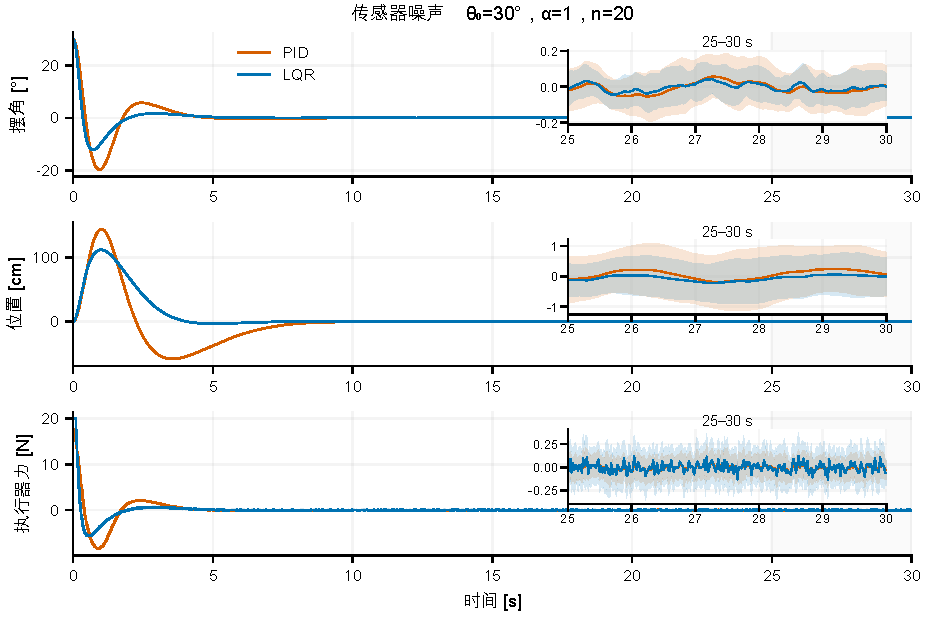
\includegraphics[width=15.8cm]{figures/noise_sensor.pdf}
\par\vspace{2pt}{\raggedright\fontsize{8.7}{11}\selectfont 图4 传感器噪声下的真实状态与执行器力（$\theta_0$=30°，$\alpha$=1，n=20）。阴影为$\pm$1样本标准差，插图放大末5 s。\par}\end{minipage}\par\vspace{3pt}
\par\noindent{\fontsize{8.7}{11}\selectfont 表4 标准传感器噪声下的末段RMS比较}\par\vspace{3pt}
{\fontsize{9.3}{11.4}\selectfont\setlength{\tabcolsep}{3pt}\renewcommand{\arraystretch}{1.1}\arrayrulecolor{tableborder}\noindent\begin{tabular}{|>{\raggedright\arraybackslash}p{4.249cm}|>{\centering\arraybackslash}p{3.965cm}|>{\centering\arraybackslash}p{3.965cm}|>{\centering\arraybackslash}p{3.871cm}|}\hline
\rowcolor{tablehead}\textbf{评价指标} & \textbf{LQR表现} & \textbf{PID表现} & \textbf{两者差距}\\\hline
摆角 RMS（°） & 0.0886 $\pm$ 0.0191 & 0.1206 $\pm$ 0.0312 & 降低 26.52\%\\\hline
位置 RMS（cm） & 0.6043 $\pm$ 0.2437 & 0.7748 $\pm$ 0.3083 & 降低 22.01\%\\\hline
执行器力 RMS（N） & 0.2158 $\pm$ 0.0091 & 0.1316 $\pm$ 0.0085 & 增加 64.01\%\\\hline
\end{tabular}}\par\vspace{3pt}
\par\noindent{\fontsize{8.7}{11}\selectfont 注：数值为20种子的均值$\pm$样本标准差；统计25—30 s；执行器力不含额外外力。}\par
LQR的摆角RMS为0.0886°，比PID的0.1206°低26.52\%；位置RMS低22.01\%。但执行器力RMS由0.1316 N增至0.2158 N，增加64.01\%；全程控制力变化率由7.5824 N/s增至12.9176 N/s，增加70.36\%。因此，本组LQR维持较小真实状态偏差的同时，控制用力与输入起伏更大。\par
本例说明，抗测量噪声表现需要联合评价状态误差与控制输入。较小的摆角波动不自动意味着较小的控制需求；若面向真实执行器，还应进一步考虑滤波、状态估计、输入变化约束及其引入的相位滞后。本文未将这些后续措施计入已有实测结论。\par
\newpage
\subsection*{4.5 噪声强度与初态范围}
\par\noindent\begin{minipage}{\linewidth}\centering
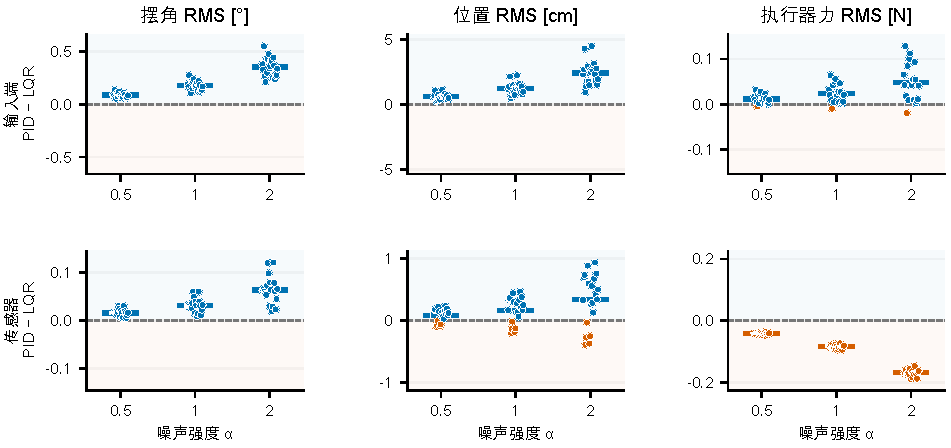
\includegraphics[width=15.7cm]{figures/noise_paired.pdf}
\par\vspace{2pt}{\raggedright\fontsize{8.7}{11}\selectfont 图5 30°初态下的同种子配对差。每点为PID$-$LQR，横杠为20个差值的均值；正值表示LQR较低，负值表示PID较低。\par}\end{minipage}\par\vspace{3pt}
\par\noindent{\fontsize{8.7}{11}\selectfont 表5 三档噪声强度下的末段摆角RMS均值}\par\vspace{3pt}
{\fontsize{9.3}{11.4}\selectfont\setlength{\tabcolsep}{3pt}\renewcommand{\arraystretch}{1.1}\arrayrulecolor{tableborder}\noindent\begin{tabular}{|>{\raggedright\arraybackslash}p{4.249cm}|>{\centering\arraybackslash}p{3.965cm}|>{\centering\arraybackslash}p{3.965cm}|>{\centering\arraybackslash}p{3.871cm}|}\hline
\rowcolor{tablehead}\textbf{噪声工况} & \textbf{LQR表现（°）} & \textbf{PID表现（°）} & \textbf{两者差距}\\\hline
输入端 $\alpha$=0.5 & 0.0677 & 0.1563 & 降低 56.67\%\\\hline
输入端 $\alpha$=1 & 0.1355 & 0.3126 & 降低 56.67\%\\\hline
输入端 $\alpha$=2 & 0.2709 & 0.6255 & 降低 56.68\%\\\hline
传感器 $\alpha$=0.5 & 0.0443 & 0.0603 & 降低 26.52\%\\\hline
传感器 $\alpha$=1 & 0.0886 & 0.1206 & 降低 26.52\%\\\hline
传感器 $\alpha$=2 & 0.1772 & 0.2411 & 降低 26.53\%\\\hline
\end{tabular}}\par\vspace{3pt}
图5按六个噪声类型与强度条件的平均摆角RMS相对改善率，试验后选取30°展示；六初态得分几乎相同，不将30°解释为明显更有利。完整六初态的36个带噪条件中，LQR的摆角与位置RMS均值均较低，但均值优势不保证每个种子都占优。\par
噪声增大时，误差随之增大，两方法相对差距在已测范围内基本一致。全部带噪运行在记录点保持|$\theta$|$<$90°，但均未达到无噪声严格四状态容差，持续随机波动与发散应分别判断。\par
\section*{5 结论}
本文完成了非线性建模、直立点线性化、串级PID与离散LQR设计及统一仿真验证。在5°—30°无噪声初态下，两者均恢复，LQR调节更快、行程和控制力平方积分更小；在两类噪声下，LQR状态误差更小，传感器噪声下则付出更大的控制力波动代价。\par
主要体会是：局部模型稳定不能代替受限非线性验证，单一指标也不能概括控制品质。工作的亮点在于固定参数公平比较、真实状态评价、同种子配对和完整归档。19项噪声协议检查及全部原始数据核验通过，两例归档重跑的三份CSV逐字节一致。后续可研究模型失配、延迟与持续外力；当前结果不构成全局稳定性证明。\par
\subsection*{参考文献}
\par\noindent{\fontsize{8.7}{11}\selectfont [1] SciPy Developers. cont2discrete. SciPy 1.9.3 Manual. 连续系统的零阶保持离散化。 \href{https://docs.scipy.org/doc/scipy-1.9.3/reference/generated/scipy.signal.cont2discrete.html}{在线资料}}\par
\par\noindent{\fontsize{8.7}{11}\selectfont [2] SciPy Developers. solve\_discrete\_are. SciPy 1.9.3 Manual. 离散代数Riccati方程求解。 \href{https://docs.scipy.org/doc/scipy-1.9.3/reference/generated/scipy.linalg.solve_discrete_are.html}{在线资料}}\par
\par\noindent{\fontsize{8.7}{11}\selectfont [3] Froze23n/cartpole. 模型与控制器源代码版本ae4bd98及2026年11月2日噪声实验归档。 \href{https://github.com/Froze23n/cartpole/tree/ae4bd98d568786a303b7da33c373f8c5e4a83461}{在线资料}}\par
\par\noindent{\fontsize{8.7}{11}\selectfont AI使用说明：使用Codex辅助推导检查、脚本编写、统计整理和报告排版。图表来自已保存的非线性仿真数据，未以生成式图像代替实验结果。}\par
\end{document}
